%%%%%%%%%%%%%%%%%%%%%%%%%%%%%%%%%%%%%%%%%%%%%%%%%%%%%%%%%%%%%%%%%%%%%%
% Problem statement
\begin{statement}[
  problempoints=100,
  timelimit=1 sekunda,
  memorylimit=512 MiB,
]{Skandalozni}

Ovo je priča o dvojici prijatelja, Stjepanu i Marinu, koji su, usprkos
rijeci Dravi, uistinu nerazdvojni. Naime, naš je dvojac nedavno kupio
zajedničko zemljište u obliku kvadrata čija stranica iznosi $N$ metara.

Obojica se žele baviti poljoprivredom, ali Stjepan želi saditi krumpire, a
Marin želi saditi kupus. Kako bi si olakšali posao, odmah su podijelili
zemljište na $N^2$ jediničnih kvadrata površine jednog kvadratnog metra.
Marin je odlučio nasumično odabrati dva (ne nužno različita) jedinična
kvadrata koji leže u istom retku te na svim kvadratima između njih posaditi
kupus.  Slično, Stjepan je odlučio nasumično odabrati dva (ne nužno
različita) jedinična kvadrata koji leže u istom stupcu te na svim kvadratima
između njih posaditi krumpir.

\begin{figure}[H]
\centering
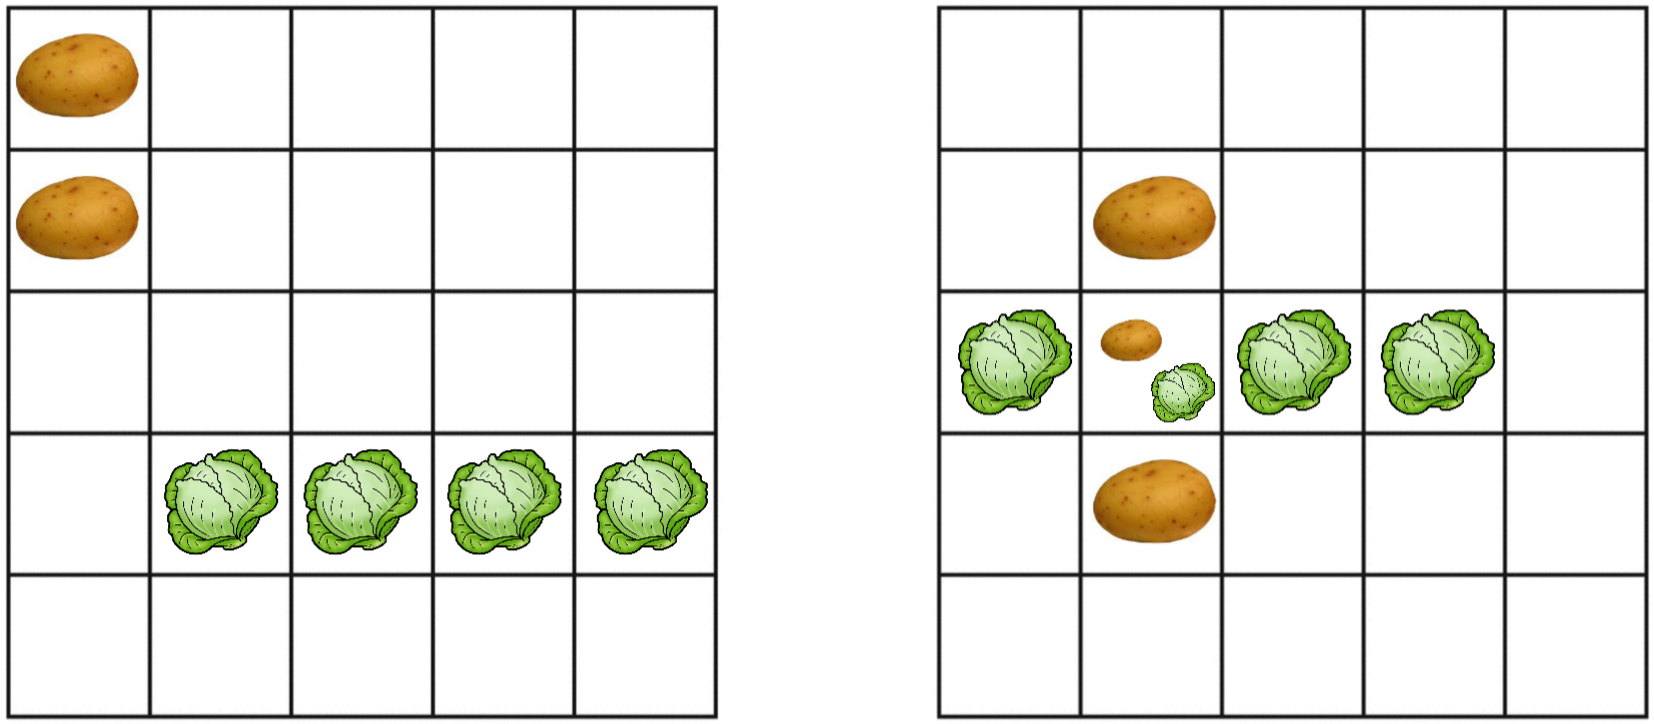
\includegraphics[width=0.53\textwidth]{img/skandal_skica.png}
\caption*{Prikaz dvaju mogućih sadnji za $N=5$. U slučaju desne sadnje dolazi do skandala.}
\end{figure}
\vspace{-0.5cm}

Naravno, ako se na nekom kvadratnom metru posadi i krumpir i kupus, nastat će
skandal. Koja je vjerojatnost da se to dogodi?

%%%%%%%%%%%%%%%%%%%%%%%%%%%%%%%%%%%%%%%%%%%%%%%%%%%%%%%%%%%%%%%%%%%%%%
% Input
\subsection*{Ulazni podaci}
U prvom je retku prirodan broj $N$ iz teksta zadatka.

%%%%%%%%%%%%%%%%%%%%%%%%%%%%%%%%%%%%%%%%%%%%%%%%%%%%%%%%%%%%%%%%%%%%%%
% Output
\subsection*{Izlazni podaci}
U jedini redak ispišite vjerojatnost da se dogodi skandal.

%%%%%%%%%%%%%%%%%%%%%%%%%%%%%%%%%%%%%%%%%%%%%%%%%%%%%%%%%%%%%%%%%%%%%%
% Scoring
\subsection*{Bodovanje}
Priznavat će se rješenja čija je apsolutna pogreška manja od $10^{-6}$.

{\renewcommand{\arraystretch}{1.4}
  \setlength{\tabcolsep}{6pt}
  \begin{tabular}{ccl}
 Podzadatak & Broj bodova & Skandalozna ograničenja \\ \midrule
  1 & 25 & $1 \le N \le 15$ \\
  2 & 25 & $1 \le N \le 1\,000$ \\
  3 & 25 & $1 \le N \le 1\,000\,000$ \\
  4 & 25 & $1 \le N \le 10^{1\,000\,000}$ \\
\end{tabular}}

%%%%%%%%%%%%%%%%%%%%%%%%%%%%%%%%%%%%%%%%%%%%%%%%%%%%%%%%%%%%%%%%%%%%%%
% Examples
\subsection*{Probni primjeri}
\begin{tabularx}{\textwidth}{X'X'X}
\sampleinputs{test/skandalozni.dummy.in.1}{test/skandalozni.dummy.out.1} &
\sampleinputs{test/skandalozni.dummy.in.2}{test/skandalozni.dummy.out.2} &
\sampleinputs{test/skandalozni.dummy.in.3}{test/skandalozni.dummy.out.3}
\end{tabularx}

%%%%%%%%%%%%%%%%%%%%%%%%%%%%%%%%%%%%%%%%%%%%%%%%%%%%%%%%%%%%%%%%%%%%%%
% We're done
\end{statement}

%%% Local Variables:
%%% mode: latex
%%% mode: flyspell
%%% ispell-local-dictionary: "croatian"
%%% TeX-master: "../hio.tex"
%%% End:
